\documentclass[11pt, a4paper]{article}

\usepackage{amsmath}
\usepackage{amsfonts} %Matheschriften
\usepackage{amssymb} %Mathesymbole
%\usepackage{mathptmx} % Einstellung für Schriften und Sonderzeichen in mathematischen Umgebungen
                        % ändert SChriftfont
\usepackage{wasysym} % Stellt diverse Sonderzeichen bereit
\usepackage{siunitx}
\usepackage{float}
\usepackage{microtype}
\usepackage{graphicx}
\usepackage{hyperref}
\usepackage{xcolor}
\usepackage[section]{placeins}
% allows for temporary adjustment of side margins
\usepackage{changepage}
\usepackage{rotating}


\usepackage[ngerman]{babel}
\addto\captionsngerman{%
 \renewcommand{\abstractname}{Einleitung}}

\title{Versuch 3: Vakuum}
\author{Team 2-13: Jascha Fricker, Benedict Brouwer}

\begin{document}
    \maketitle

    \tableofcontents

    \newpage

    \section{Einleitung}
    In diesem Versuch wurden die verschiedenen Eigenschaften einer Vakuumpumpe untersucht. Dazu musste aber zuerst das Druckmessgerät kallibriert werden.

    \section{Theorie}

    \paragraph{Piranimeter}
    Die Wärmeleitfähigkeit eines Gases ist bei kleinen Drücken abhängig vom dessen Druck. Damit einhergehend ist die benötigte Leistung um einen sich im Messaufbau befindlichen Wolframdraht auf Temperatur zu halten Druckabhängig. Diese Abhängigkeit kann genuzt werden indem Wiederstand und Stromstärke gemessen werden um Rückschlüsse auf den Druck zu ziehen.

    \paragraph{Saugvermögen} Bei konstantem Druck kann das Saugvermögen $S$ durch die (negative) Volumenänderung $\Delta V_L$
    \begin{align}
        \underbrace{\frac{d(p_L V_L)}{dt}}_{konst} &= Q_S = Q_V = p_V \cdot S \\
        \Rightarrow S &= \left\lvert\frac{p_L \cdot \Delta V}{p_V \cdot \Delta t}\right\rvert \label{eq:saugvermoegen}
    \end{align}
    bestimmt werden. Dabei ist $Q_s$ die Saugleisung bei Luftdruck $p_L$ und $Q_V$ die Saugleisung an der Vakuumpumpe mit Druck $p_V$.

    \paragraph{effektives Saugvermögen}
    Durch verschieden Strömungshindernisse kann das das volle Saugvermögen der Pumpe meist nicht ausgereitzt werden. Daraus folg ein kleineres effektiveres Saugvermögen
    \begin{align}
        \frac{1}{S_eff} = \frac{1}{S} + \frac{1}{L_1} + \frac{1}{L_2} + \dots \label{seff}\\
    \end{align}

    Lokal kann der Druck beim auspumpen auch durch die Formel
    \begin{align}
        p\left(t\right) = p_0 \cdot exp\left(- \frac{S_{eff}}{V} \cdot t\right)
    \end{align}
    beschrieben werden, wobei $p_0$ geeignet gewählt werden muss.
    Theoretisch kann der Leitwert der Kapillare mit Durchmesser $d$ und Länge $l$ bei viskoser Strömungs (mittlere freie Weglänge $\lambda \ll d$) durch die Formel
    \begin{align}
        L = \frac{\pi d^4}{128 \cdot \eta \cdot l} \cdot \frac{}{} \label{leitvisk}
    \end{align}
    und bei molekularer Strömung ($\lambda \gg d$) mit der Formel
    \begin{align}
        L = 121 \si{\meter\per\second} \cdot \frac{d^3}{l}
    \end{align}
    berechnet werden, unter Voraussetzung, dass das Medium Luft auf Raumtemperatur ist.

    Für den Leitwert mehrerer hintereinandergeschalteter Strömungshindernisse gilt die Formel
    \begin{align}
        \frac{1}{L_{ges}} = \frac{1}{L_1} + \frac{1}{L_2}
    \end{align}






    \section{Ergebnisse}
    \subsection{Kallibrierung des Piranimeters}
    Durch die Messwerte des ersten Experiments konnte der Graph mit dem Verhältins zwischen Druck $p$ und Strom $I$ aufgestellt werden. Durch diesen wurde eine abschnittweise definierte Kurve gefittet, um in den nächsten Abschnitten durch den gemessenen Strom Rückschlüsse auf den vorherschenden Druck ziehen zu können.
    \begin{figure}[h]
        \centering
        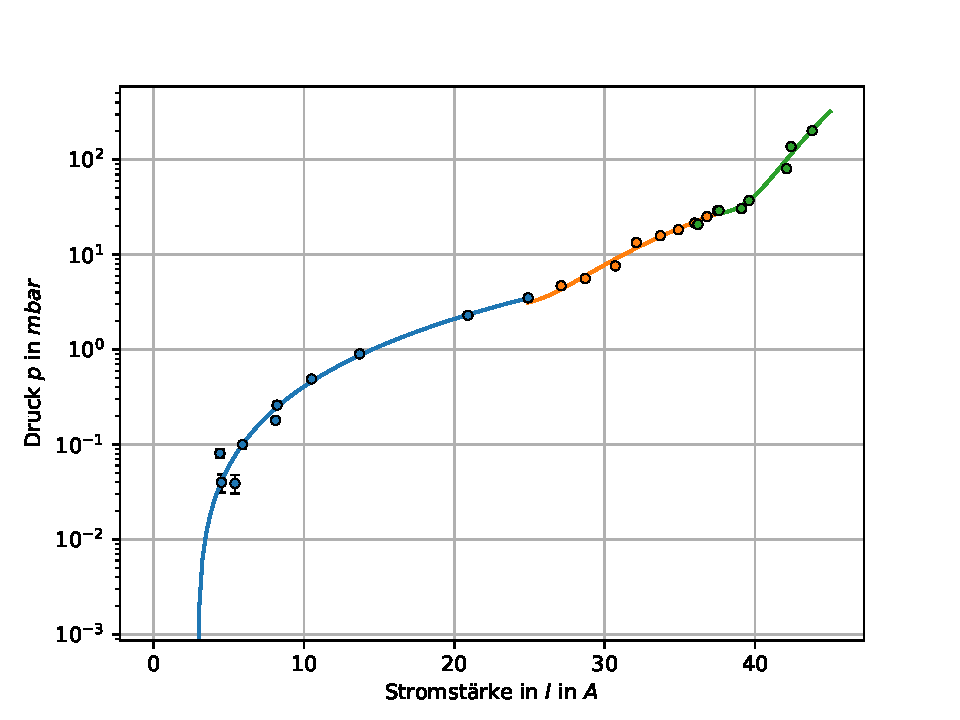
\includegraphics[width=0.8\textwidth]{Kallibrierung.pdf}
        \caption{Kallibrierung des Piranimeters}
        \label{fig:piranim}
    \end{figure}
    \subsection{Leistung des Piranimeters}
    Aus dem Wiederstand des Piranimeters und der gemessenen Stromstärke kann mit $P_{pir} = R \cdot I^2$ die Leistung berechnet werden und mit den Daten des Membranmanometers geplottet werden. Dabei lässt sich erkennen, dass die Leistung sich im Bereich von 0 bis 4 \si{\milli\bar} annäherend proportional zum Druck verhält. 
    \begin{figure}[h]
        \centering
        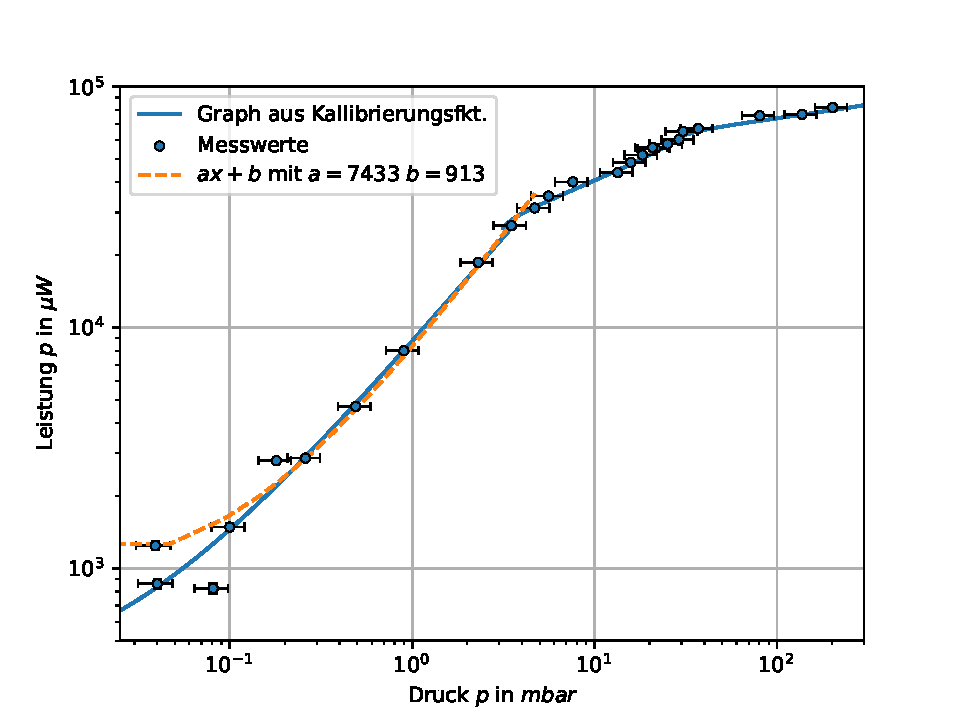
\includegraphics[width=0.8\textwidth]{Pp_Graph.pdf}
        \caption{Leistung des Piranimeters}
        \label{fig:Pzup}
    \end{figure}



    \subsection{Saugvermögen}
    Durch auspumpen eines Beweglichen Kolbens und Messung der Kolbengeschwindigkeit konnte mit Formel \ref{eq:saugvermoegen}  das Saugvermögen der Pumpe $S$ bei verschiedenen Drücken $p$ bestimmt werden. Die errechneten Werte sind in der Tabelle \ref{tab:./VAK/saug} aufgeführt.
    \input{saug.txt}
    Die Angabe von $3,5 \si{\meter\cubed\per\hour}$ ist wahrscheinlich die minimale Saugleistung bei Normdruck, so erklähren sich die Werte \> $3,5 \si{\meter\cubed\per\hour}$. 
    Die geringere Saugleistung bei niedrigerem Druck lässt sich vermutlich erklären durch mehr Lecks bei niedrigerem Druck welche einen Verhältinsmäsig größeren Einfluss auf die Saugleistung haben und durch eine schlechteren Effizienz der Pumpe je kleiner der Druck.
    %Dass die Saugleistung bei niedrigerem Druck abfällt, ist dadurch erklärbar, dass die Pumpe und der Aufbau bei niedrigerem Druck mehr Luft durch Lecks fließt und die Pumpe wahrscheinlich nicht mehr so effizient arbeitet.

    \subsection{effektives Saugvermögen}

    Durch den Schlauch und die Kapillaren wird das Saugvermögen gemindert. In Graph \ref{fig:effSaug} wird der Druck beim Auspumpvorgang des $3.0(1) l$ Behälters geplottet. Aus den angelegten Geraden kann anschließend die effektive Saugleistung, die in Tabelle X ausgeführt wird, bestimmt werden. Diese unterscheidet zwischen viskoser Strömung, bei der die mittlere freie Weglänge viel kürzer ist als der Durchmesser des Rohr, also der Effekt einer Kollision mit der Gefäßwand unwesentlich ist, und molekularer Strömung, bei der die Weglänge viel größer als der Durchmesser ist, also Kollisionen mit der Wand wichtig, aber jene zwischen den Molekülen unwesentlich sind.

    \begin{figure}[h]
        \centering
        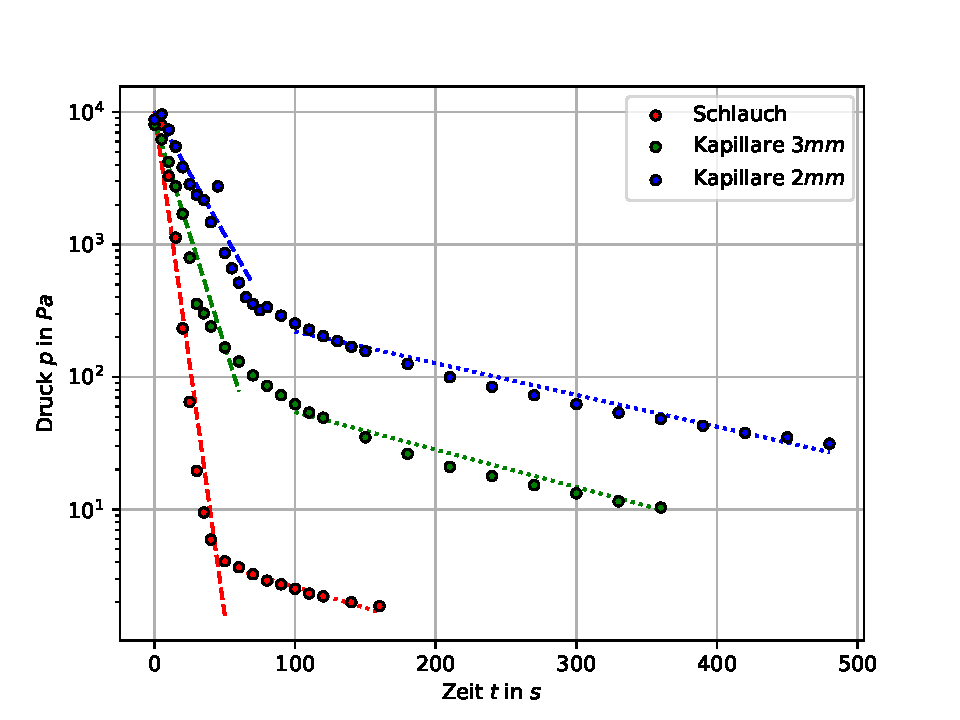
\includegraphics[width=0.8\textwidth]{Saugver.pdf}
        \caption{effektives Saugvermögen}
        \label{fig:effSaug}
    \end{figure}

    \input{seff.txt}

    

    \subsubsection{Theoretische Leitwerte}
    In der Tabelle \ref{tab:./VAK/tabelle} werden die theoretisch berechneten Leitwerte und effektive Saugleistungen der verschiedenen Konstellationen aus Schlauch und Kapillare dargestellt. Dabei wurde eine nominale Saugleistung von $S = 3,7 \si{\meter\per\hour}$ angenommen.
    \input{tabelle.txt}
    Die ermessenen Werte ähneln den theoretischen berechneten Leitwerten. Da aber die Messmethode sehr ungenau ist und die Berechnung durch den fit viel Ungenauigkeiten enthält, waren die relativ großen Abweichungen zu erwarten.

    \subsection{Fragen}
    \paragraph{Frage 1}
    Bei viskoser Strömung ist die mittlere freie Weglänge viel kürzer ist als der Durchmesser des Rohr. D.h. der Effekt einer Kollision mit der Gefäßwand ist unwesentlich. Bei molekularer Strömunghingegen ist die mittlere freie Weglänge viel größer als der Durchmesser, also sind Kollisionen mit der Wand wichtig, aber jene zwischen den Molekülen unwesentlich.

    
    \paragraph{Frage 2}
    Wir nehmen an, dass durch den kleinen Durchmesser so wenig Luft fließt, dass fur die ganze Zeit von $t = 600s$ ein viskoser Fluss angenommen werden kann. Es folgt mit Formel \ref{leitvisk} und \ref{seff}:
    \begin{align}
        L_{1mm} = \frac{\pi \cdot 1 \si{\milli\meter}^4}{128 \cdot 1,82 \cdot 10^{-5} \si{\kilogram\per\milli\second} \cdot 9,5 \si{\centi\metre} \cdot 957 \si{\hecto\pascal}} = 1,358 \cdot 10^{-6} \si{\meter\cubed\per\second} \\
        S_{eff} = \frac{1}{\frac{1}{9,72 \cdot 10^{-4} \si{\meter\cubed\per\second}} + \frac{1}{1,358 \cdot 10^{-6} \si{\meter\cubed\per\second}}} = 1,357 \cdot 10^{-6} \si{\meter\cubed\per\second} \\
        p(600 \si{\second}) = 957 \si{\hecto\pascal} \cdot exp\left(-\frac{1,357 \cdot 10^{-6} \si{\meter\cubed\per\second}}{3 \si{\liter}} \cdot 600 \si{\second}\right) = 730 \si{\hecto\pascal}
    \end{align}
    Da bei $730 \si{\hecto\pascal}$ noch viskose Strömung vorliegt, ist unsere Annahme begründet.

    \paragraph{Frage 3}
    Wenn wir annehmen, dass die Formel
    \begin{align}
        p \cdot V = N \cdot k_b \cdot T
    \end{align}
    gilt und $T = 273,15K$ einsetzen, ergibt sich ein Druck von
    \begin{align}
        p = \frac{N \cdot k_b \cdot T}{V} = \frac{1 \cdot 1,380649 \cdot 10^{-23} \si{\joule\per\kelvin} \cdot 237,15 \si{\kelvin}}{1 \si{\meter\cubed}} = 3,274 \cdot 10^{-21} \si{\pascal} \,.
    \end{align}

    \bibliographystyle{plain}
    \bibliography{literature}

\end{document}